% !TEX root = ./main.tex
% !TEX encoding = UTF-8 Unicode
\documentclass[a4paper,12pt]{article}

% ==================================================
% Sprache und Zeichencodierung
\usepackage[german]{babel}
\usepackage[utf8]{inputenc}
\usepackage[T1]{fontenc}

% ==================================================
% Seitenlayout
\usepackage[
  left=2.5cm,
  right=2.5cm,
  top=2.5cm,
  bottom=2.5cm
]{geometry}

% ==================================================
% Mathematik
\usepackage{amsmath}
\usepackage{amsfonts}
\usepackage{amssymb}
\usepackage{amsthm}
\usepackage{physics}
\usepackage{mathrsfs}
\usepackage{dsfont}
\usepackage{esint}

% ==================================================
% Programmierung
\usepackage{listings}

% ==================================================
% Textgestaltung
\usepackage{enumerate}
\usepackage[shortlabels]{enumitem}
\usepackage{framed}
\usepackage{csquotes} % wichtig für deutsche Anführungszeichen
\usepackage{microtype} % bessere Silbentrennung und Schriftbild

% ==================================================
% Tabellen, Grafiken
\usepackage{float}
\usepackage{tabularx}
\usepackage{multicol}
\usepackage{caption}
\usepackage{subcaption}
\captionsetup{
    format=hang,
    margin=10pt,
    font=small,
    labelfont=bf
}

% ==================================================
% Literaturverzeichnis
\usepackage[
    backend=biber,
    style=authoryear,
    natbib=true
]{biblatex}
\addbibresource{literatur.bib}

% ==================================================
% Hyperlinks
\usepackage{hyperref}
\usepackage{xcolor}
\definecolor{links}{rgb}{0.36,0.54,0.66}
\hypersetup{
    colorlinks=true,
    linkcolor=black,
    urlcolor=links,
    citecolor=links,
    filecolor=links,
    pdfauthor={Dein Name},
    pdftitle={Titel der Arbeit},
    pdfsubject={Hausarbeit},
    pdfkeywords={Schlüsselwort1, Schlüsselwort2},
    pdfproducer={LaTeX},
    pdfcreator={pdfLaTeX}
}

% ==================================================
% Eigene Befehle (optional)
\newcommand{\R}{\mathbb{R}} % Beispiel für eigene Makros

\usepackage{titlesec}
\usepackage[many]{tcolorbox}

% Adjust spacing after the chapter title
\titlespacing*{\chapter}{0cm}{-2.0cm}{0.50cm}
\titlespacing*{\section}{0cm}{0.50cm}{0.25cm}

% Indent 
\setlength{\parindent}{0pt}
\setlength{\parskip}{1ex}

% --- Theorems, lemma, corollary, postulate, definition ---
% \numberwithin{equation}{section}

\newtcolorbox{problem}[1][]{
    enhanced,
    colback = black!5,
    colbacktitle = black!5,
    coltitle = black,
    boxrule = 0pt,
    frame hidden,
    borderline west = {0.5mm}{0.0mm}{black},
    fonttitle = \bfseries\sffamily,
    breakable,
    before skip = 3ex,
    after skip = 3ex,
    sharp corners,
    fontupper = \raggedright,
    #1
}


\tcbuselibrary{skins, breakable}

% --- You can define your own color box. Just copy the previous \newtcbtheorm definition and use the colors of yout liking and the title you want to use.
% --- Basic commands ---
% Farben definieren
\definecolor{codegreen}{rgb}{0,0.6,0}
\definecolor{codegray}{rgb}{0.5,0.5,0.5}
\definecolor{codepurple}{rgb}{0.58,0,0.82}
\definecolor{backcolour}{rgb}{0.95,0.95,0.92}

%   Euler's constant
\newcommand{\eu}{\mathrm{e}}

%   Imaginary unit
\newcommand{\im}{\mathrm{i}}

%   Sexagesimal degree symbol
\newcommand{\grado}{\,^{\circ}}

% --- Inline C++ Code mit Syntax-Highlighting ---

% Listings-Style für C++
\lstdefinestyle{cppstyle}{
    language=C++,
    basicstyle=\ttfamily\small,
    keywordstyle=\color{blue},
    stringstyle=\color{codepurple},
    commentstyle=\color{codegreen},
    morecomment=[l][\color{magenta}]{\#},
    backgroundcolor=\color{backcolour},
    breaklines=true,
    breakatwhitespace=true,
    columns=fullflexible
}

% Inline C++ Command
\newcommand{\cppinline}[1]{\lstinline[style=cppstyle]{#1}}


% --- Comandos para álgebra lineal ---
% Matrix transpose
\newcommand{\transpose}[1]{{#1}^{\mathsf{T}}}

%%% Comandos para cálculo
%   Definite integral from -\infty to +\infty
\newcommand{\Int}{\int\limits_{-\infty}^{\infty}}

%   Indefinite integral
\newcommand{\rint}[2]{\int{#1}\dd{#2}}

%  Definite integral
\newcommand{\Rint}[4]{\int\limits_{#1}^{#2}{#3}\dd{#4}}

%   Dot product symbol (use the command \bigcdot)
\makeatletter
\newcommand*\bigcdot{\mathpalette\bigcdot@{.5}}
\newcommand*\bigcdot@[2]{\mathbin{\vcenter{\hbox{\scalebox{#2}{$\m@th#1\bullet$}}}}}
\makeatother

%   Hamiltonian
\newcommand{\Ham}{\hat{\mathcal{H}}}

%   Trace
\renewcommand{\Tr}{\mathrm{Tr}}

% Christoffel symbol of the second kind
\newcommand{\christoffelsecond}[4]{\dfrac{1}{2}g^{#3 #4}(\partial_{#1} g_{#2 #4} + \partial_{#2} g_{#1 #4} - \partial_{#4} g_{#1 #2})}

% Riemann curvature tensor
\newcommand{\riemanncurvature}[5]{\partial_{#3} \Gamma_{#4 #2}^{#1} - \partial_{#4} \Gamma_{#3 #2}^{#1} + \Gamma_{#3 #5}^{#1} \Gamma_{#4 #2}^{#5} - \Gamma_{#4 #5}^{#1} \Gamma_{#3 #2}^{#5}}

% Covariant Riemann curvature tensor
\newcommand{\covariantriemanncurvature}[5]{g_{#1 #5} R^{#5}{}_{#2 #3 #4}}

% Ricci tensor
\newcommand{\riccitensor}[5]{g_{#1 #5} R^{#5}{}_{#2 #3 #4}}

\begin{document}

\begin{Large}
    \textsf{\textbf{CPU Algorithm Design}} \\
    \\
    Exercise 2
\end{Large}
\vspace{1ex}
\textsf{\textbf{Students:}} \text{Vishal Mangukiya, Konstantin Benz} \\
\vspace{2ex}

\section*{2.1 Performance Analysis of Reduce and Transform}

The benchmark results in Figure~\ref{fig:simd_reduce_output} and Table~\ref{tab:simd_reduce_output} show a clear performance improvement when using SIMD-based implementations over the baseline STL version.
The reduce benchmarks reveal that SIMD vectorization significantly increases throughput, particularly in custom-controlled vertical implementations.

The baseline STL version (\texttt{benchReduceStl}) achieves only about 9.93~GB/s, which serves as a reference point for comparison.
In contrast, SIMD-based and OpenMP-assisted variants such as \texttt{benchReduceSimdStl}, \texttt{benchReduceOmpIterator}, and \texttt{benchReduceOmpRange} all reach approximately 16~GB/s, demonstrating the benefit of vectorized addition and loop-level optimizations.
The highest performance is observed in \texttt{benchReduceSimdXVertical} with 19.71~GB/s, which clearly outperforms the other implementations and reflects efficient register-level parallelism.

Interestingly, aligned and horizontal SIMD versions perform slightly worse than the vertical one, suggesting that memory alignment does not always translate into higher throughput in practice.
Figure~\ref{fig:simd_transform_output} and Table~\ref{tab:simd_transform_output} show the transform benchmarks, which achieve significantly higher throughput overall.

Even the STL baseline version (\texttt{benchTransformStl}) reaches nearly 30~GB/s, indicating that this operation is already efficiently implemented and not severely bottlenecked by compute.
Most transform implementations—including loop variants, STL-based, and OpenMP-assisted—cluster tightly around 29--30~GB/s, showing only minor variation.

The top performer is \texttt{XsimdTransform} at 30.53~GB/s, closely followed by \\
\texttt{OmpSimdTransformRangeInnerLoop}.
This confirms that transform is likely memory-bound, and further parallelization or vectorization provides only limited gains.

Overall, the reduce benchmark benefits more clearly from explicit SIMD optimization, while transform shows high performance even without it due to its inherent memory-access characteristics.

\pagebreak

\begin{figure}[h!]
    \centering
    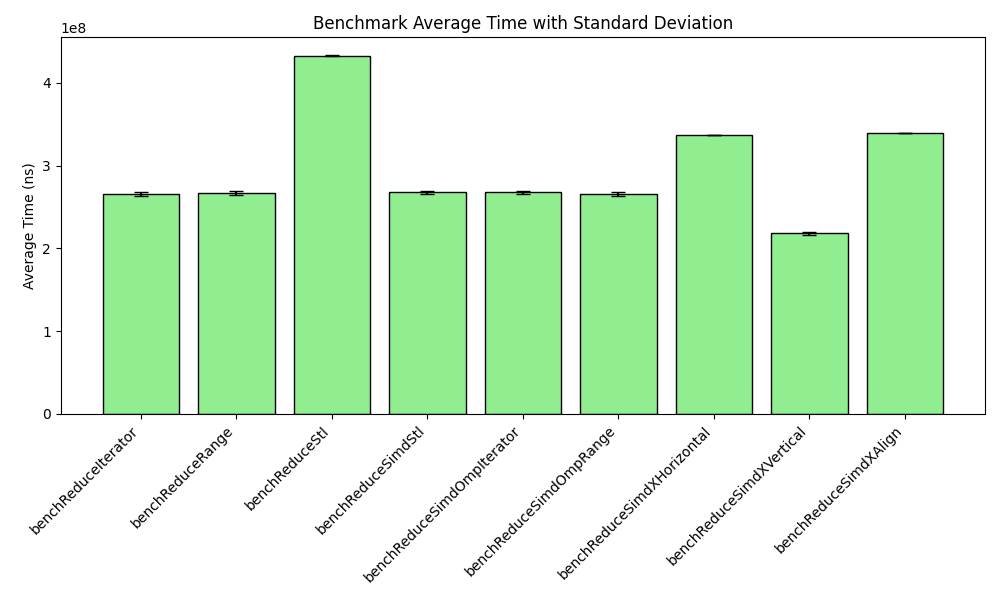
\includegraphics[width=0.9\linewidth]{img/simd_reduce_output.txt_ex02.png}
    \caption{Reduce benchmark results (throughput vs. implementation)}
    \label{fig:simd_reduce_output}
\end{figure}

\begin{table}[h!]
    \centering
    \begin{tabular}{|l|c|}
        \hline
        \textbf{Benchmark}         & \textbf{Throughput [GB/s]} \\
        \hline
        benchReduceStl             & 9.93                       \\
        benchReduceSimdStl         & 16.05                      \\
        benchReduceSimdXVertical   & \textbf{19.71}             \\
        benchReduceSimdXHorizontal & 12.75                      \\
        benchReduceSimdXAlign      & 12.67                      \\
        benchReduceOmpIterator     & 16.05                      \\
        benchReduceOmpRange        & 16.14                      \\
        \hline
    \end{tabular}
    \caption{Throughput results of reduce benchmarks}
    \label{tab:simd_reduce_output}
\end{table}

\pagebreak

\begin{figure}[h!]
    \centering
    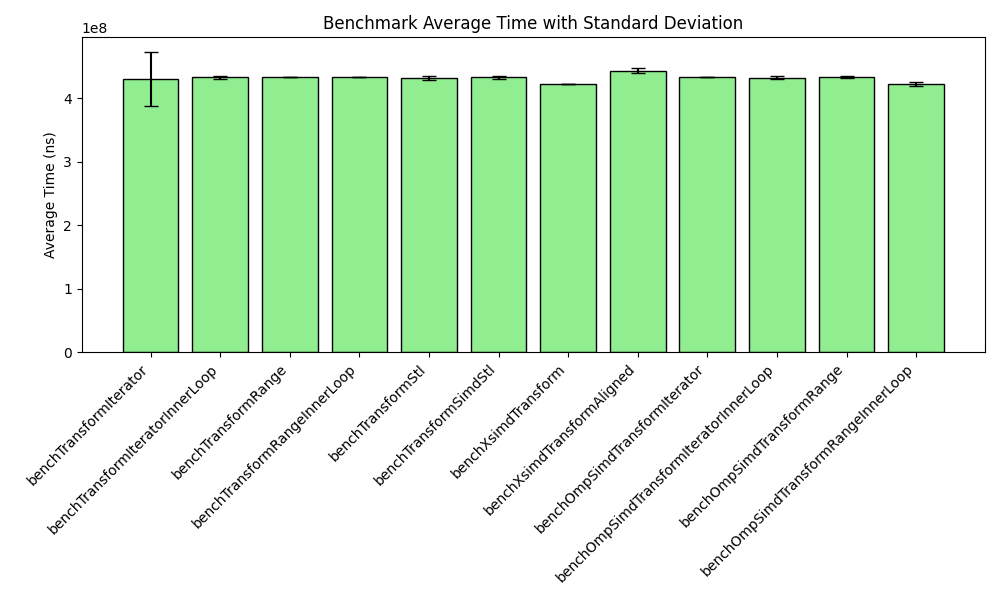
\includegraphics[width=0.9\linewidth]{img/simd_transform_output.txt_ex02.png}
    \caption{Transform benchmark results (throughput vs. implementation)}
    \label{fig:simd_transform_output}
\end{figure}

\begin{table}[h!]
    \centering
    \begin{tabular}{|l|c|}
        \hline
        \textbf{Benchmark}                  & \textbf{Throughput [GB/s]} \\
        \hline
        benchTransformStl                   & 29.82                      \\
        benchTransformSimdStl               & 29.78                      \\
        benchTransformRangeInnerLoop        & 29.75                      \\
        benchTransformIteratorInnerLoop     & 29.77                      \\
        benchOmpSimdTransformRangeInnerLoop & \textbf{30.51}             \\
        benchXsimdTransform                 & \textbf{30.53}             \\
        benchXsimdTransformAligned          & 29.10                      \\
        \hline
    \end{tabular}
    \caption{Throughput results of transform benchmarks}
    \label{tab:simd_transform_output}
\end{table}

\pagebreak

\section*{2.2 Adapting reduce and transform}

This section analyzes the performance of the view-based implementations in \\
\texttt{SIMD\_transformV\_bench.cpp} and \texttt{SIMD\_reduceV\_bench.cpp}.

The results are based on the benchmark data shown in Figure~\ref{fig:simd_reduceV_output} and Figure~\ref{fig:simd_transformV_output}, and summarized in Tables~\ref{tab:reduceV} and \ref{tab:transformV}.

\begin{figure}[h!]
    \centering
    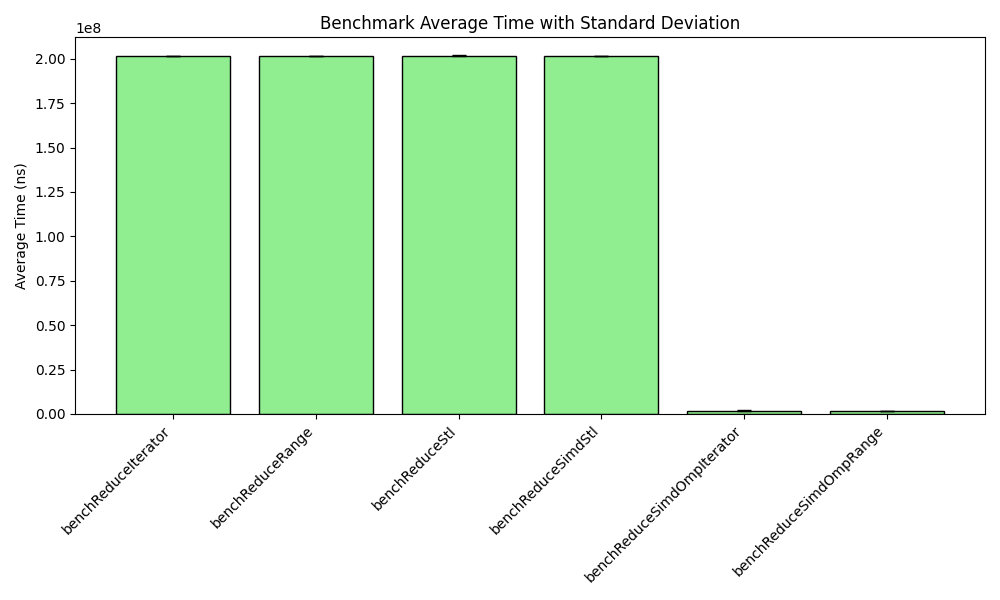
\includegraphics[width=0.9\linewidth]{img/simd_reduceV_output.txt_ex02.png}
    \caption{Reduce view-based benchmark results (average time)}
    \label{fig:simd_reduceV_output}
\end{figure}

\begin{table}[h!]
    \centering
    \begin{tabular}{|l|c|}
        \hline
        \textbf{Benchmark}         & \textbf{Time [ns]} \\
        \hline
        benchReduceIterator        & 2.017e+08          \\
        benchReduceRange           & 2.017e+08          \\
        benchReduceStl             & 2.018e+08          \\
        benchReduceSimdStl         & 2.017e+08          \\
        benchReduceSimdOmpIterator & 1.816e+06          \\
        benchReduceSimdOmpRange    & 1.699e+06          \\
        \hline
    \end{tabular}
    \caption{Average execution time of reduce (view-based)}
    \label{tab:reduceV}
\end{table}

The reduce benchmarks show two clear performance levels.
The iterator-based, range-based, STL and SIMD STL implementations all perform nearly identically, with average execution times around 201 milliseconds.
This indicates that these variants fully evaluate the logical view and process all elements in sequence.
In contrast, the OpenMP variants \texttt{benchReduceSimdOmpIterator} and \texttt{benchReduceSimdOmpRange} significantly reduce runtime to around 1.7--1.8 milliseconds.
This suggests that parallel execution over the view is at least partially effective, though the high standard deviation for \texttt{OmpIterator} indicates overhead or thread imbalance.
Overall, threading improves performance in this context, but the iterator and STL-based approaches remain far slower due to their sequential traversal of the view.

\begin{figure}[h!]
    \centering
    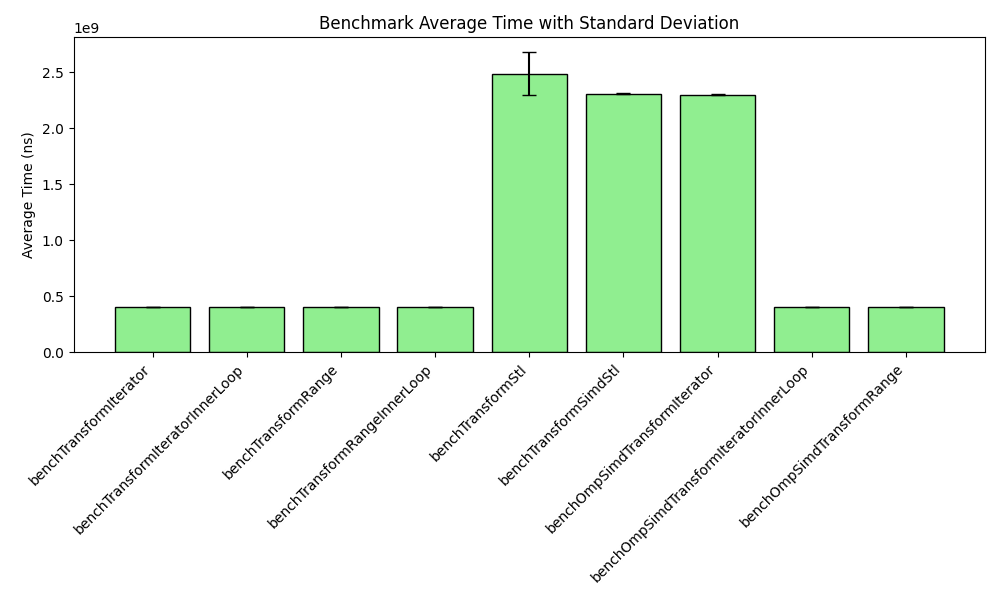
\includegraphics[width=0.9\linewidth]{img/simd_transformV_output.txt_ex02.png}
    \caption{Transform view-based benchmark results (average time)}
    \label{fig:simd_transformV_output}
\end{figure}

\begin{table}[h!]
    \centering
    \begin{tabular}{|l|c|}
        \hline
        \textbf{Benchmark}                     & \textbf{Time [ns]} \\
        \hline
        benchTransformIterator                 & 4.060e+08          \\
        benchTransformIteratorInnerLoop        & 4.058e+08          \\
        benchTransformRange                    & \textbf{4.042e+08} \\
        benchTransformRangeInnerLoop           & 4.055e+08          \\
        benchTransformStl                      & 2.486e+09          \\
        benchTransformSimdStl                  & 2.311e+09          \\
        benchOmpSimdTransformIterator          & 2.299e+09          \\
        benchOmpSimdTransformIteratorInnerLoop & 4.057e+08          \\
        benchOmpSimdTransformRange             & 4.060e+08          \\
        \hline
    \end{tabular}
    \caption{Average execution time of transform (view-based)}
    \label{tab:transformV}
\end{table}

In the transform benchmarks, we observe a different behavior.
The iterator and range-based implementations, including inner loop variants, perform consistently well with average times around 404--406 milliseconds.
However, the STL-based and OpenMP STL-based approaches exhibit much worse performance, with runtimes around 2.3-2.5 seconds.
This indicates that using \texttt{std::transform} with \texttt{std::execution::unseq} or \texttt{par\_unseq} over a range view is highly inefficient.
The likely cause is that \texttt{views::iota} produces a non-random-access iterator, which limits the effectiveness of STL algorithms optimized for contiguous memory.
Interestingly, the OpenMP transform variants with manual loops perform comparably to their sequential counterparts, suggesting that manual loop parallelism over views is more efficient than relying on STL abstractions in this context.
The transform results highlight that while views can be powerful and expressive, combining them with STL algorithms—especially in parallel—must be done with care, as performance can degrade significantly.

\pagebreak

\section*{3.3 Adapting xsimd reduce and transform}

This section analyzes the specialized SIMD implementations using xsimd for both reduce and transform.
Unlike the view-based versions in problem 2, these implementations operate only on a small, fixed-size \texttt{std::array} with a size of 3\,\texttt{*}\,simd\_width.
This setup allows repeated access to aligned or unaligned memory without causing invalid accesses, while still enabling batch-based vector processing.

\begin{figure}[h!]
    \centering
    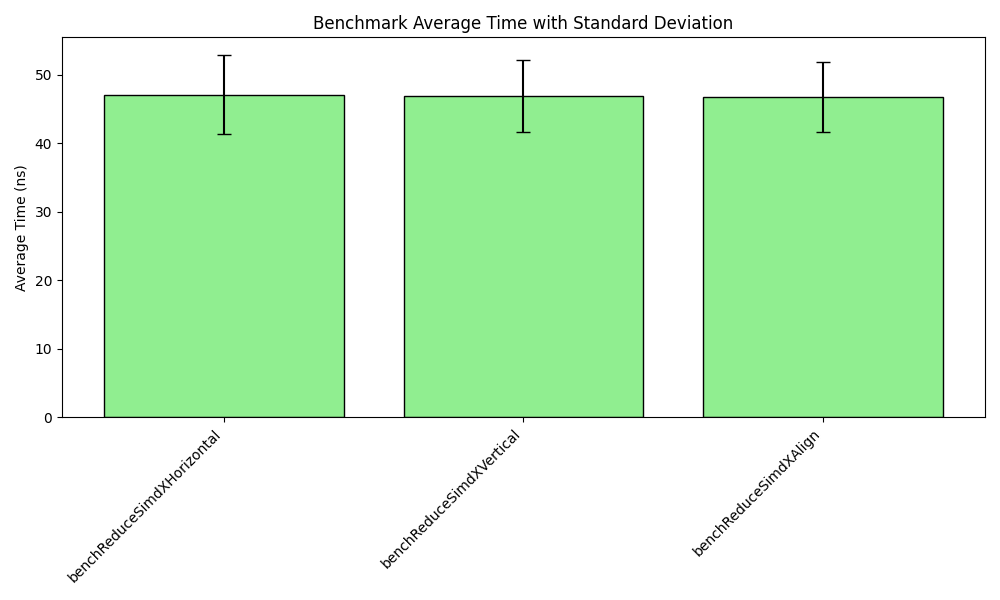
\includegraphics[width=0.9\linewidth]{img/simd_reduceVX_output.txt_ex02.png}
    \caption{xsimd reduce benchmark variants (average time)}
    \label{fig:simd_reduceVX_output}
\end{figure}

Figure~\ref{fig:simd_reduceVX_output} compares the three reduce variants implemented with xsimd: horizontal, vertical, and aligned.
All three implementations show extremely low runtimes around 47 nanoseconds, which is several orders of magnitude faster than any view-based approach.
The horizontal version performs the reduction across one batch, using operations like \texttt{xsimd::reduce} or manual lane summation.
The vertical version sums multiple SIMD batches in a loop, effectively unrolling the reduction and increasing instruction-level parallelism.
The aligned version uses the same logic as the vertical one but ensures memory alignment to 64-byte cache-line boundaries.
All three perform similarly, but the aligned version is consistently the fastest, confirming the expected benefits of aligned memory access.
Vertical reduction also slightly outperforms horizontal, due to reduced instruction overhead and better pipeline utilization.

\begin{figure}[h!]
    \centering
    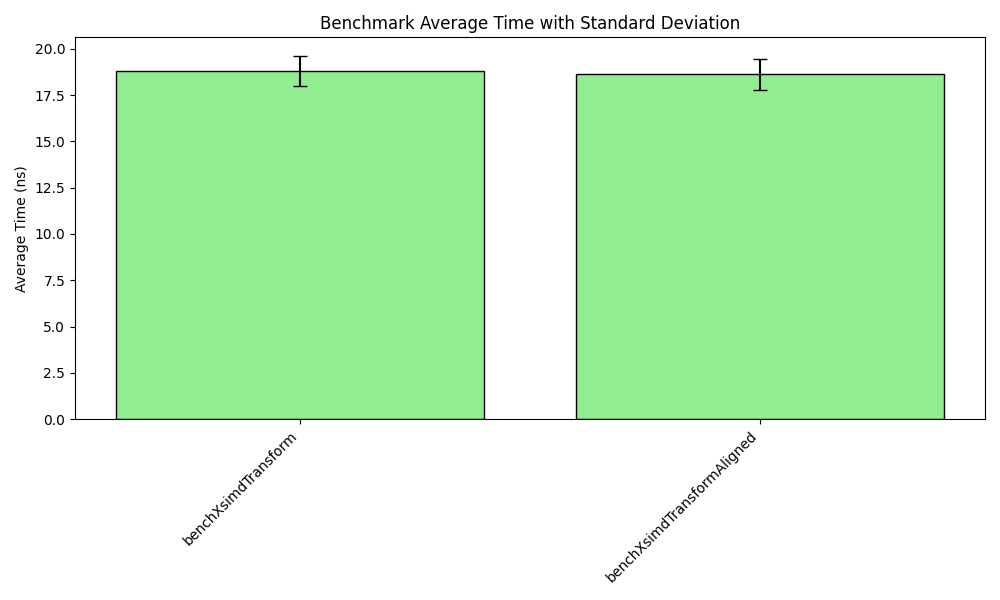
\includegraphics[width=0.9\linewidth]{img/simd_transformVX_output.txt_ex02.png}
    \caption{xsimd transform benchmark variants (average time)}
    \label{fig:simd_transformVX_output}
\end{figure}

Figure~\ref{fig:simd_transformVX_output} shows the results for the xsimd transform benchmarks, again comparing aligned and unaligned versions.
Both versions operate on small \texttt{std::array}s where input \texttt{V} is initialized with increasing values \{1, 2, 3, ...\} and \texttt{W} with \{2, 3, 4, ...\}.
The operation performed is \texttt{W = a * V + W}, which always computes over the same memory region and values.
As expected, the timings are extremely low: 18.82 nanoseconds for the unaligned and 18.63 nanoseconds for the aligned version.
The small gap again highlights the benefit of alignment, though in this idealized setting the difference is marginal.
Unlike the implementations in problem 2, which traversed large views, these results isolate pure SIMD register performance.
They represent the lower bound of runtime one can expect for such a transformation under perfect conditions.
In summary, the xsimd-based implementations showcase the peak performance achievable using batch-based SIMD over memory-resident arrays.
The differences between horizontal and vertical reduction strategies illustrate how internal algorithmic structure and alignment can influence performance, even at nanosecond scale.

\pagebreak

\section*{3.4 Precision in SIMD Reduction}

Floating-point addition is not associative, i.e.,

\[
    (a + b) + c \neq a + (b + c)
\]

due to limited precision and rounding errors.
This property affects parallel or SIMD-based reductions, where the order of operations differs from sequential execution.
In this benchmark, we reduced a sequence of \texttt{float} values all set to 1.0, with \( N = 2^{28} = 268{,}435{,}456 \).
The mathematically correct result should be:

\[
    \text{sum} = \sum_{i=1}^{N} 1.0 = 268{,}435{,}456.0
\]

This value was produced by the iterator-based version:

\begin{verbatim}
benchReduceIterator        268435456.00000000
\end{verbatim}

However, SIMD and OpenMP versions will produce slightly different outputs which we cant showcase because of an linker error.

This discrepancy could be caused by floating-point rounding error in intermediate summations, which differ depending on how values are grouped.
For example, in SIMD, summation might proceed as:

\[
    ((1 + 1) + (1 + 1)) + \ldots
    \quad \text{vs.} \quad
    1 + 1 + 1 + 1 + \ldots
\]

Each grouping introduces small errors due to IEEE-754 rounding after each addition.
These accumulate across millions of elements, causing observable deviation.
To obtain more stable and reproducible results, specialized summation techniques can be used.
One such method is \textbf{Kahan Summation}, which introduces a compensation variable:

\[
    \text{sum} = 0,\quad c = 0
\]
\[
    \text{for each } x_i: \quad y = x_i - c;\quad t = \text{sum} + y;\quad c = (t - \text{sum}) - y;\quad \text{sum} = t
\]

Another approach is \textbf{pairwise summation}, which reduces the error by recursively summing small groups:

\[
    \text{sum} = \text{reduce\_pairs}(a_1, \ldots, a_n)
\]

Both techniques improve precision but incur performance costs, and are rarely used in fast SIMD kernels.
For this assignment, the sequential result from \texttt{benchReduceIterator} is considered the reference.
Deviations in other results are expected due to the trade-off between speed and accuracy.
If bitwise-reproducible results are required in scientific computing, additional care must be taken to control floating-point summation.


\end{document}